\subsection{Decomposition}
\subsubsection{Method}
Given a system of FDE
\begin{equation}
\begin{cases}
    \mathcal{D}_c^\alpha y(t)=f(t,y)&\\ y(0)=y_0\quad t\in[0,T]&
\end{cases}
\end{equation}\label{eq:FDESystemDeco}
the Adomian Decomposition method for fractional differential equations, presented in \cite{momani2007numerical}, starts by splitting $f$ as follows
\begin{equation}
    f(t,y)=g(t)+\mathbf{A}y+h(t,y)
\end{equation}
Where $g$ is the part of each equation that only depends on $t$; $\mathbf{A}y$ is the linear components of the equations and $h$ is the nonlinear part. Applying the Riemann-Liouville operator (section \ref{sec:RL}) to both sides of equation \ref{eq:FDESystemDeco}, we obtain
\begin{equation*}
    J^\alpha\mathcal{D}_c^\alpha y(t)=J^\alpha g(t)+J^\alpha\mathbf{A}y+J^\alpha h(t,y)
\end{equation*}
The left side of the equation can be calculated using theorem \ref{theo:rightinverse}. Therefore
\begin{equation*}
    y(t) = \sum_{r=0}^{m-1}\dfrac{y_{(r)}t^r}{r!}+ J^\alpha g(t)+J^\alpha\mathbf{A}y+J^\alpha h(t,y)
\end{equation*}
Since $\mathbf{y}$ is an unknown vector of solutions, it is approximated through a power series of functions as follows:
\begin{equation*}
    y(t)=\sum_{r=0}^\infty x_r(t)
\end{equation*}
That yields the next recursive scheme:
\begin{equation}\label{eq:recur_deco}
    \begin{split}
        x_0&=\sum_{r=0}^{m-1}\dfrac{y_{(r)}t^r}{r!}+J^\alpha g(t)\\
        x_{k+1}&=J^\alpha \mathbf{A}x_k+J^\alpha \tilde{h}_k\left(t,\sum_{r=0}^kx_j(t)\right)
    \end{split}
\end{equation}
Where $\tilde{h}_k$ is the Adomian polynomial, described by
\begin{equation}
    \tilde{h}_k\left(t,\sum_{r=0}^{k}x_j(t)\right)=\dfrac{1}{k!}\left[\dfrac{d^k}{d\lambda^k}h\left(t,\sum_{j=0}^{k}\lambda^jx_j(t)\right)\Bigg|_{\lambda=0}\right]
\end{equation}


\begin{exmp}\label{ex:deco}
Solve the following the fractional initial value problem using Decomposition, with $y(0)=1$ and $y'(0)=0$.
\begin{equation}
    \mathcal{D}_c^{1.25}y(t)=-y(t)
\end{equation}
\end{exmp}
Carrying out some analytic operations, the exact solution is given by
\begin{equation}
    y(t) = E_{1.25,\,1}(-t^{1.25})=\sum_{k=0}^{\infty}\dfrac{(-1)^kt^{1.25k}}{\Gamma(1.25k +1)} 
\end{equation}
Notice that this example is the same as the one that was developed in the previous section: example \ref{ex:adam}.

The Decomposition method was executed with different number of polynomials in order to show how the exact solution is better approximated for more polynomials. The plot for the results are shown in figure \ref{fig:deco_frac}; on the other hand, table \ref{tab:exDeco} shows the numeric approximation in certain values of $t$. Note that all approximations stabilize around the same value.

\begin{table}[H]
\centering
\begin{tabular}{cccccc}
\hline
\textbf{Time}    & \boldmath{$N=1$} & \boldmath{$N=5$} & \boldmath{$N=10$} & \boldmath{$N=15$} & Exact   \\ \hline
\boldmath{$t=0$} & 1.0000           & 1.0000           & 1.0000            & 1.0000            & 1.0000  \\
\boldmath{$t=1$} & 0.1174           & 0.3655           & 0.3655            & 0.3655            & 0.3655  \\
\boldmath{$t=2$} & -1.0992          & -0.0074          & 0.0036            & 0.0036            & 0.0036  \\
\boldmath{$t=3$} & -2.4847          & -0.3103          & -0.0988           & -0.0989           & -0.0989 \\
\boldmath{$t=4$} & -3.9928          & -1.7581          & -0.0891           & -0.0926           & -0.0926 \\
\boldmath{$t=5$} & -5.5990          & -8.1585          & 0.0098            & -0.0625           & -0.0625 \\
\boldmath{$t=6$} & -7.2882          & -29.0799         & 0.8027            & -0.0397           & -0.0385 \\
\boldmath{$t=7$} & -9.0494          & -84.6072         & 6.6218            & -0.0508           & -0.0246 \\ \hline
\end{tabular}
\caption{Numerical results using Decomposition algorithm for different polynomials}
\label{tab:exDeco}
\end{table}

\begin{figure}[H]
    \centering
    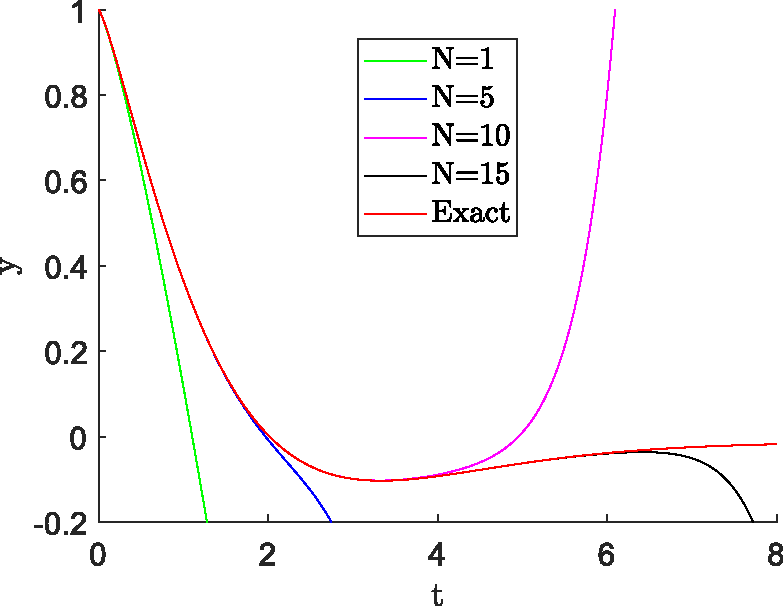
\includegraphics[scale=0.5]{files/frac_deco.pdf}
    \caption{Decomposition using different number of polynomials.}
    \label{fig:deco_frac}
\end{figure}

\subsection{Phase Variables: Fractional Case}
Suppose we have the multi-term fractional differential equation
\begin{equation}
    \begin{cases}
    \mathcal{D}_c^{\alpha_n}y(t)=f\left(t,y,\mathcal{D}_c^{\alpha_1}y,\mathcal{D}_c^{\alpha_2}y,\dots,\mathcal{D}_c^{\alpha_{n-1}}y\right)&\\
    y(0)=y_0,\,\dots,y^{(m-1)}(0)= y_{(m-1)}\quad t\in[0,T]
    \end{cases}
\end{equation}
    where $m=\ceil{\alpha_n}$ and $0<\alpha_{1}<\alpha_{2}<\ldots<\alpha_{n}$. We select new orders $\tilde{\alpha}_{1}, \ldots, \tilde{\alpha}_{n}$ such that
    \[\begin{array}{l}{\text { (a) } \tilde{\alpha}_{1}, \ldots, \tilde{\alpha}_{n} \text { must be rational numbers, }} \\ {\text { (b) }\left\lceil\alpha_{n}\right\rceil=\left\lceil\tilde{\alpha}_{n}\right\rceil} \\ {\text { (c) } \operatorname{gcd}\left(1, \tilde{\alpha}_{1}, \ldots, \tilde{\alpha}_{n}\right) \text { should be as large as possible, }} \\ {\text { (d) }\left|\alpha_{j}-\tilde{\alpha}_{j}\right| \text { should be as small as possible for all } j}\end{array}\]

    We build the approximated system of FDEs with \[\gamma :=\operatorname{gcd}\left(1, \tilde{\alpha}_{1}, \ldots, \tilde{\alpha}_{n}\right)\qquad\tilde{N} :=\frac{\tilde{\alpha}_{n}}{\gamma}\]
    \begin{equation}
    \begin{cases}
    
    \mathcal{D}_c^{\gamma} x_{0} =x_{1} &\\[5pt]
    \mathcal{D}_c^{\gamma} x_{1} =x_{2} &\\
    \qquad\vdots &\\
    \mathcal{D}_c^{\gamma} =x_{\tilde{N}-1} &\\[5pt]
    \mathcal{D}_c^{\gamma} =f\left(t, x_{0}, x_{\tilde{\alpha}_{1} / \gamma}, \ldots, x_{\tilde{\alpha}_{n-1} / \gamma}\right) \end{cases}
    \end{equation}
    \begin{equation}
    x _ { j } ( 0 ) = \begin{cases} { y _ { ( j \gamma ) }   } & { \text { for } j \gamma \in \mathbb { N } _ { 0 } } \\ { 0  } & { \text { else } } \end{cases}
    \end{equation}
